\chapter{Creating a Coincidence Detector In Simulation} \label{chap:creating-detector}
Developing the AND gate posed a significant challenge as it is highly dependent on specific geometric configurations for proper operation. 
While it is acknowledged that such a coincidence detector is feasible, the focus of our investigation is on the stability of such simulations in response to environmental changes and the practicality of implementing them in a real environment.
Although we acknowledge that building this in a simulation is possible, the focus of this paper is to determine the stability of the simulation in response to environmental changes and the practicality of implementing them in a real environment. 


\section{Unsuccessful Detector}\label{unsuccessful-detector}
\begin{figure}
    \centering
    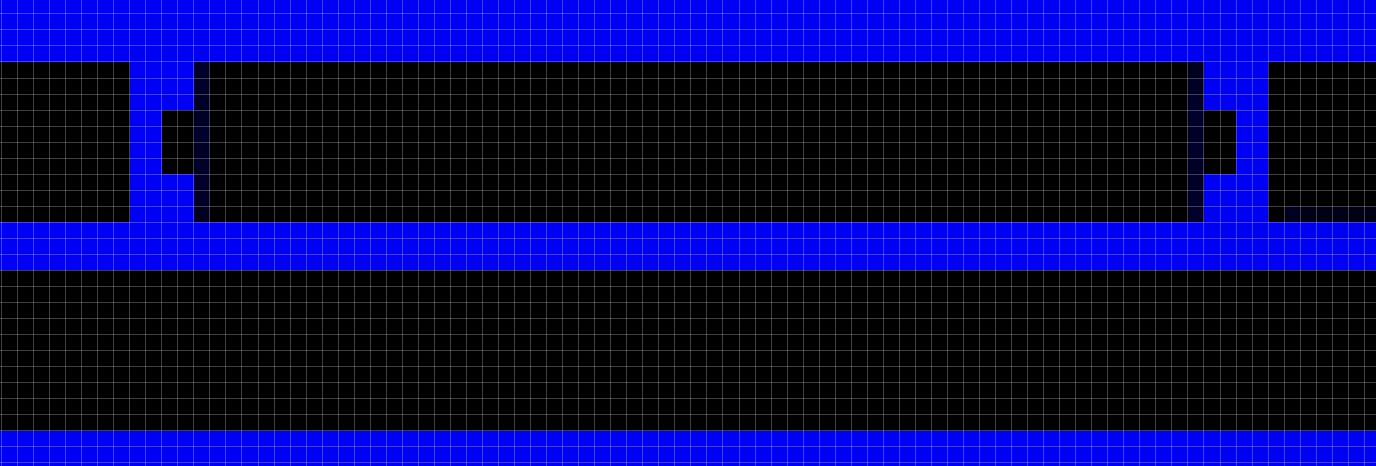
\includegraphics[width=0.75\linewidth]{image7.png}
    \caption{Initial Coincidence Detector Configuration}
    \label{fig:unsuccessful-config-and-gate}
\end{figure}
\begin{table}[h]
\centering
\begin{tabular}{|c|c|c|c|c|}
\hline
Width & Gap=1px & Gap=2px & Gap=3px & Gap=4px \\ \hline
w=1px & NP & NP & NP & NP \\ \hline
w=2px & NP & NP & NP & NP \\ \hline
w=3px & AP & NP & NP & NP \\ \hline
w=4px & AP & AP & NP & NP \\ \hline
w=5px & AP & AP & NP & NP \\ \hline
w=6px & AP & AP & NP & NP \\ \hline
w=7px & AP & AP & NP & NP \\ \hline
w=8px & AP & AP & NP & NP \\ \hline
w=9px & AP & AP & NP & NP \\ \hline
w=11px & AP & AP & NP & NP \\ \hline
w=12px & AP & AP & NP & NP \\ \hline
w=13px & AP & AP & NP & NP \\ \hline
\end{tabular}
\caption{Results of the experiment showing the relationship between conductor width and gap size.}
\label{table:experiment-results}
\end{table}
In our investigation, we focus on three controllable variables: 
\begin{itemize}
    \item the width of the conductor
    \item its length before the gap.
\end{itemize}
The detector configuration is shown in Figure \ref{fig:unsuccessful-config-and-gate}.
The primary question we seek to answer is how the width of the conductor influences the functionality of the gates. Specifically, our experiment aims to identify an optimal conductor width that enables the "if" gate to function correctly. This gate's operation relies on two conductors positioned closely, requiring a precise amount of force to facilitate signal transmission from one to the other. This force is generated by the collision of two waves. However, current configurations fail due to the conductors being excessively proximate.

For the purposes of this experiment, we define three outcomes based on the interaction between the waves and the conductors:
- Always pass (AP): The signal always passes through the gap.
- Never pass (NP): The signal never passes through the gap.
- Collision pass (CP): The signal passes through the gap only upon collision of waves.

The CP outcome is of particular interest as it represents the desired state for computational functionality.

Initial tests did not yield CP outcomes, suggesting a potential discrepancy in the values of $\phi_{\text{active}}$ versus $\phi_{\text{passive}}$. Adjusting $\phi_{\text{active}}$ to a more aggressive value of 0.035f resulted in CP outcomes for every gap of 3px, marking a significant deviation from the default value of 0.054 proposed in prior literature. This finding prompts further investigation into the range of values between 0.035 and 0.054 to identify a flexible operational window. 

A successful configuration identified involves a long charge, a gap of 3px, and a $\phi_{\text{active}}$ value of 0.035. Further exploration is required to determine a viable configuration for a gap of 2px.

Additionally, our observations reveal notable differences in wave behavior depending on orientation; specifically, vertical wave propagation exhibits distinct properties compared to horizontal propagation. A particularly intriguing observation is that waves originating off-center tend to accelerate asymmetrically, favoring one direction over the other, and resulting in a higher likelihood of collision.

\section{Successful Detector}

Section \ref{unsuccessful-detector} led to the conclusion that there must be more parameters in play that prevent the detector from functioning, and it was later found that the height of the diode pin on the active medium of the coincidence detector. 
Following this, it was discovered that by setting the pins higher or lower, we change from where the wave approaches the detector medium, allowing for a finer adjustment of the opration. This created the first successful detector, seen in Figure \ref{fig:first-successful-detector}.

\begin{figure}
    \centering
    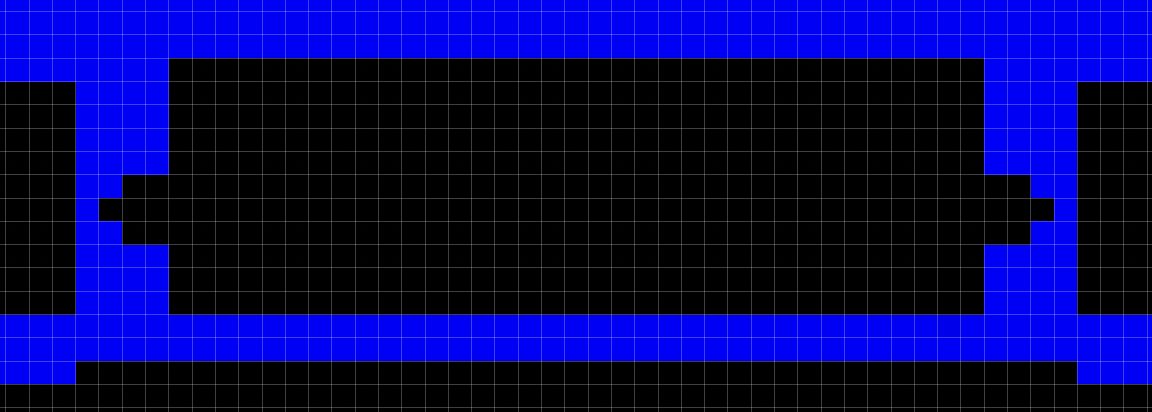
\includegraphics[width=0.75\linewidth]{image9.png}
    \caption{First Successful Coincidence Detector}
    \label{fig:first-successful-detector}
\end{figure}


Normally the wave also depends on where it is coming from, but we can ignore that in our case because we are using diodes at entry of the detector medium. Diodes add a new entry point for the incoming wave, so the incoming direction does not really matter. 

There is still a small problem with this design where if two waves meet around the centre, none of them gets enough momentum to develop fully and they don't have enough concentration to diffuse into the result substrate, this can be solved by increasing the length of the detector medium to allow for both waves to form, so later designs have a longer detector medium, like in Figure \ref{fig:and-gate}

The length of the coincidence detector depends on two factors:
\begin{enumerate}
    \item The minimum distance apart they need to be from each other while still allowing for the waves to form inside the detector.
    \item The minimum distance apart they have to be, so that the centre is still usable for collusion.
\end{enumerate}